\chapter{Wireless Security}\label{wireless-security}

\section{Intro to Wireless Network
Security}\label{intro-to-wireless-network-security}

\begin{itemize}
\item
  Although SECURITY is important in ALL NETWORKS, it is even more
  essential in WIRELESS NETWORKS
\item
  Because WIRELESS SIGNALS are not contained within a WIRE, any DEVICE
  within range of the signal can receive traffic
\item
  In WIRED NETWORKS, traffic is often only ENCRYPTED when sent over an
  UNTRUSTED NETWORK such as the INTERNET
\item
  In WIRELESS NETWORKS, it is VERY important to ENCRYPT traffic sent
  between the WIRELESS CLIENTS and the AP
\item
  We will cover THREE MAIN CONCEPTS:

  \begin{itemize}
  \tightlist
  \item
    AUTHENTICATION
  \item
    ENCRYPTION
  \item
    INTEGRITY
  \end{itemize}
\end{itemize}

\section{Authentication}\label{authentication}

\begin{itemize}
\tightlist
\item
  All CLIENTS must be AUTHENTICATED before they can associate with an AP
\item
  In a corporate setting, only TRUSTED USERS / DEVICES should be given
  ACCESS to the NETWORK

  \begin{itemize}
  \tightlist
  \item
    In corporate settings, a separate SSID which doesn't have ACCESS to
    the corporate NETWORK can be provided for GUEST USERS
  \end{itemize}
\item
  Ideally, CLIENTS should also AUTHENTICATE the AP to avoid associating
  with a malicious AP
\item
  There are MULTIPLE WAYS to AUTHENTICATE:

  \begin{itemize}
  \tightlist
  \item
    PASSWORD
  \item
    USERNAME / PASSWORD
  \item
    CERTIFICATES
  \end{itemize}
\end{itemize}

\begin{figure}
\centering
\pandocbounded{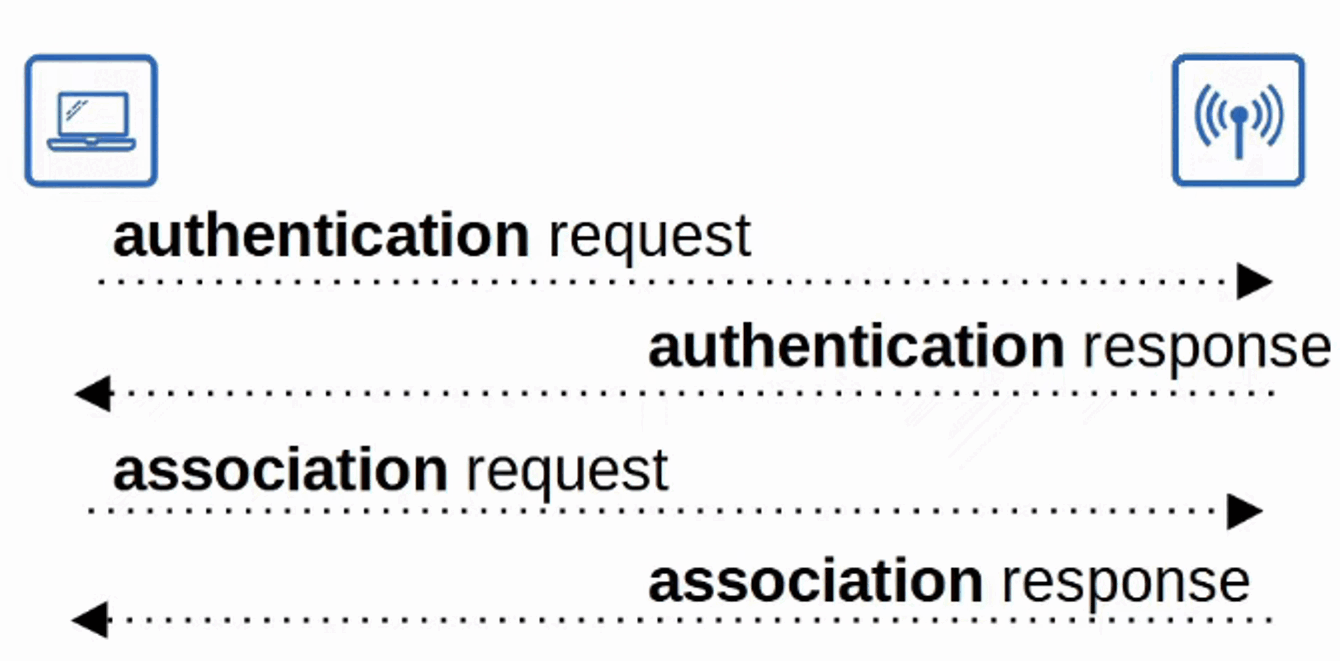
\includegraphics[keepaspectratio,alt={image}]{images/60-wireless-security/img-001.png}}
\end{figure}

\section{Encryption}\label{encryption}

\begin{itemize}
\tightlist
\item
  Traffic sent between CLIENTS and APs should be ENCRYPTED so that it
  can't be read by anyone except the AP and the CLIENT
\item
  There are many possible PROTOCOLS that can be used to ENCRYPT traffic
\item
  All DEVICES on the WLAN will use the same PROTOCOL, however each
  CLIENT will use a unique ENCRYPTION / DECRYPTION KEY so that other
  DEVICES can't read its traffic
\item
  A ``GROUP KEY'' is used by the AP to ENCRYPT traffic that it wants to
  send to all of its clients

  \begin{itemize}
  \tightlist
  \item
    All of the CLIENTS associated with the AP keep that key so they can
    DECRYPT the traffic
  \end{itemize}
\end{itemize}

\section{Integrity}\label{integrity}

\begin{itemize}
\tightlist
\item
  As explained in the ``SECURITY FUNDAMENTALS'' video of the course,
  INTEGRITY ensures that the message is not modified by a third-party
\item
  The message that is sent by the SOURCE HOST should be the same as the
  message that is received by the DESTINATION HOST
\item
  A MIC (Message Integrity Check) is added to the message to help
  protect their INTEGRITY.
\end{itemize}

\begin{figure}
\centering
\pandocbounded{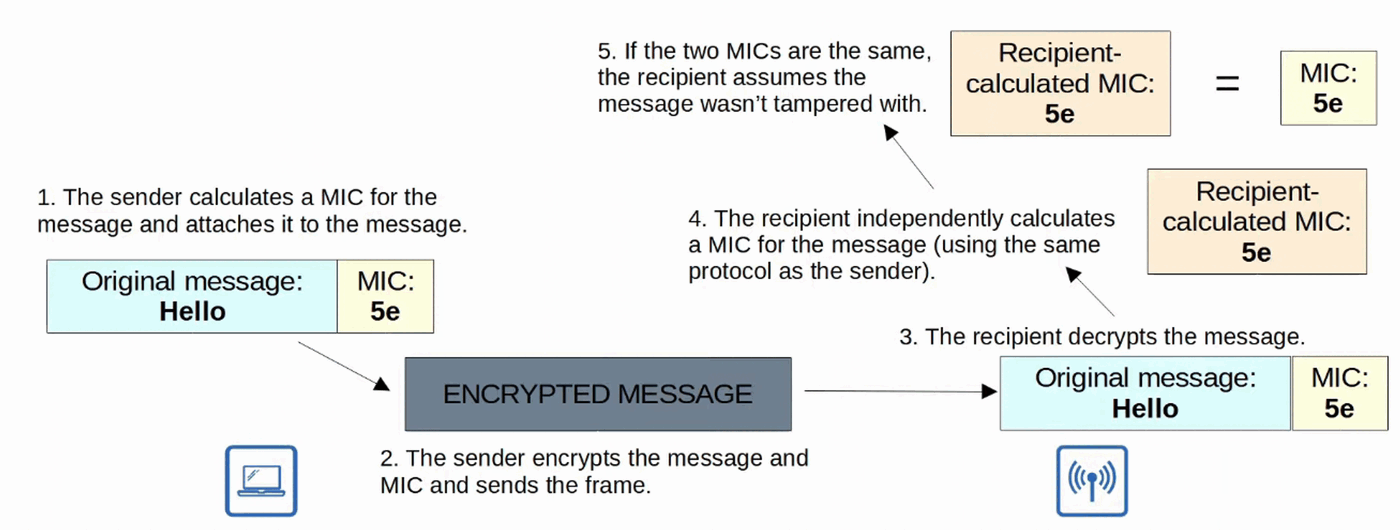
\includegraphics[keepaspectratio,alt={image}]{images/60-wireless-security/img-002.png}}
\end{figure}

\section{Authentication Methods}\label{authentication-methods}

The original 802.11 STANDARD included TWO OPTIONS for AUTHENTICATION:

\begin{itemize}
\tightlist
\item
  OPEN AUTHENTICATION

  \begin{itemize}
  \tightlist
  \item
    The CLIENT sends an AUTHENTICATION REQUEST and the AP just accepts
    it
  \item
    The is clearly NOT a SECURE AUTHENTICATION method
  \item
    After the CLIENT is AUTHENTICATED and associated with the AP, it's
    possible to require the USER to AUTHENTICATE via other methods
    before ACCESS to the NETWORK is granted (ie: Starbucks WI-FI)
  \end{itemize}
\item
  WEP (Wired Equivalent Privacy)

  \begin{itemize}
  \tightlist
  \item
    WEP is used to provide both AUTHENTICATION and ENCRYPTION of
    WIRELESS traffic
  \item
    For ENCRYPTION, WEP uses the RC4 ALGORITHM
  \item
    WEP is a ``SHARED-KEY'' PROTOCOL, requiring the SENDER and RECEIVER
    to have the same KEY
  \item
    WEP KEYS can be 40 bits or 104 bits in length
  \item
    The above KEYS are combined with a 24-bit ``IV'' (INITIALIZATION
    VECTOR) to bring the total length to 64 bits or 128 bits
  \item
    WEP ENCRYPTION is NOT SECURE and can easily be cracked
  \item
    WEP can be used for AUTHENTICATION like this:
  \end{itemize}
\end{itemize}

\begin{figure}
\centering
\pandocbounded{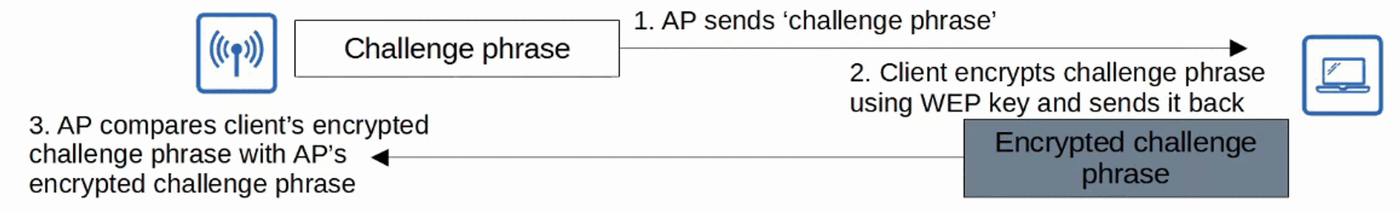
\includegraphics[keepaspectratio,alt={image}]{images/60-wireless-security/img-003.png}}
\end{figure}

EAP (Extensible Authentication Protocol)

\begin{itemize}
\tightlist
\item
  EAP is an AUTHENTICATION FRAMEWORK
\item
  It defines a STANDARD SET of AUTHENTICATION FUNCTIONS that are used by
  the various \emph{EAP METHODS}
\item
  We will look at FOUR EAP METHODS:

  \begin{itemize}
  \tightlist
  \item
    LEAP
  \item
    EAP-FAST
  \item
    PEAP
  \item
    EAP-TLS
  \end{itemize}
\item
  EAP is integrated with \textbf{802.1X} which provides \emph{PORT-BASED
  NETWORK ACCESS CONTROL}
\end{itemize}

\textbf{802.1X} is used to limit NETWORK ACCESS for CLIENTS connected to
a LAN or WLAN until they AUTHENTICATE

There are \textbf{THREE MAIN ENTITIES} in 802.1X:

\begin{itemize}
\tightlist
\item
  SUPPLICANT : The DEVICE that wants to connect to the NETWORK
\item
  AUTHENTICATOR : The DEVICE that provides access to the NETWORK
\item
  AUTHENTICATION SERVER (AS) : The DEVICE that receives CLIENT
  credentials and PERMITS / DENIES ACCESS
\end{itemize}

\begin{figure}
\centering
\pandocbounded{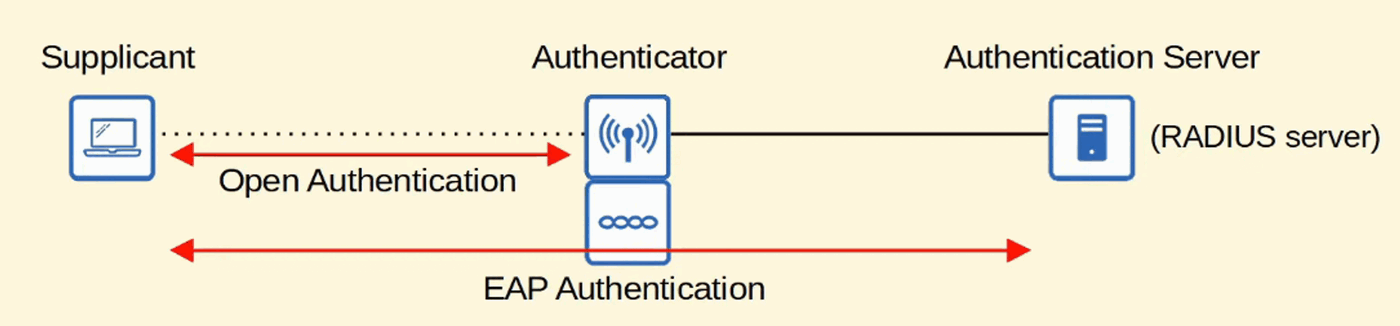
\includegraphics[keepaspectratio,alt={image}]{images/60-wireless-security/img-004.png}}
\end{figure}

\begin{itemize}
\tightlist
\item
  LEAP (Lightweight EAP)

  \begin{itemize}
  \tightlist
  \item
    LEAP was developed by Cisco an an improvement over WEP
  \item
    CLIENTS must provide a USERNAME and PASSWORD to AUTHENTICATE
  \item
    In addition, \emph{MUTUAL AUTHENTICATION} is provided by both the
    CLIENT and SERVER sending a CHALLENGE PHRASE to each other.
  \item
    DYNAMIC WEP KEYS are used, meaning that the WEP KEYS are changed
    frequently
  \item
    Like WEP, LEAP is considered vulnerable and should not be used
    anymore
  \end{itemize}
\end{itemize}

\begin{figure}
\centering
\pandocbounded{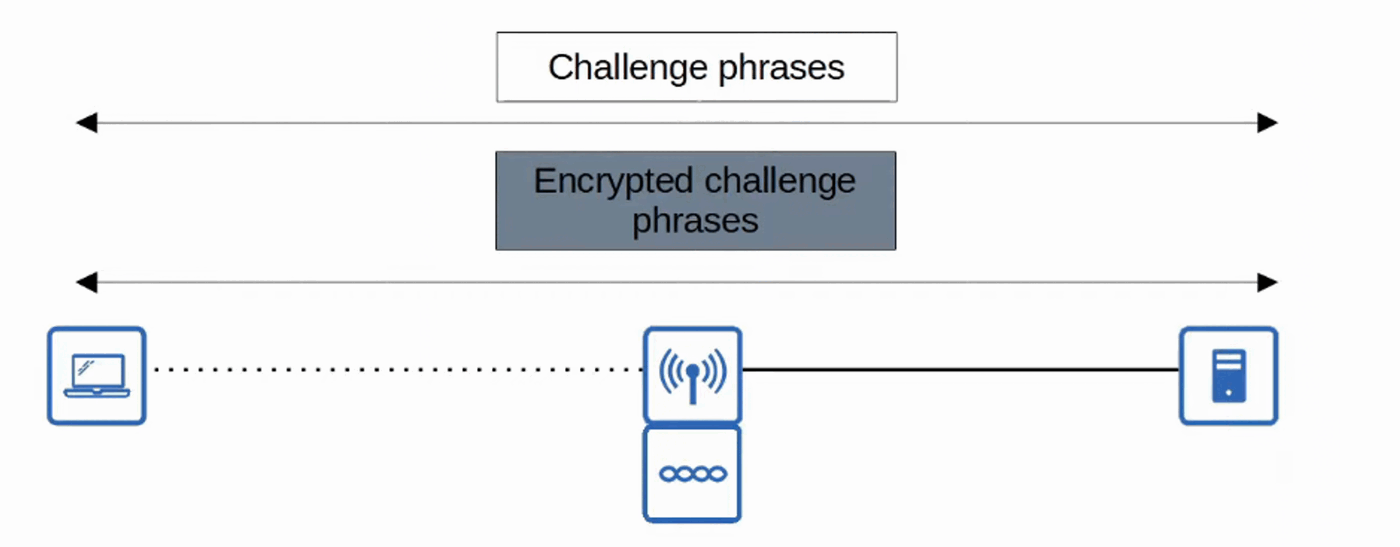
\includegraphics[keepaspectratio,alt={image}]{images/60-wireless-security/img-005.png}}
\end{figure}

\begin{itemize}
\tightlist
\item
  EAP-FAST (EAP FLEXIBLE AUTHENTICATION via SECURE TUNNELING)

  \begin{itemize}
  \tightlist
  \item
    EAP-FAST was also developed by Cisco
  \item
    Consists of THREE PHASES:

    \begin{itemize}
    \tightlist
    \item
      A PAC (PROTECTED ACCESS CREDENTIAL) is generated and passed from
      SERVER to CLIENT
    \item
      A SECURE TLS TUNNEL is established between the CLIENT and
      AUTHENTICATION SERVER
    \item
      Inside of the SECURE (ENCRYPTED) TLS TUNNEL, the CLIENT and SERVER
      communicated further to AUTHENTICATE / AUTHORIZE the CLIENT
    \end{itemize}
  \end{itemize}
\end{itemize}

\begin{figure}
\centering
\pandocbounded{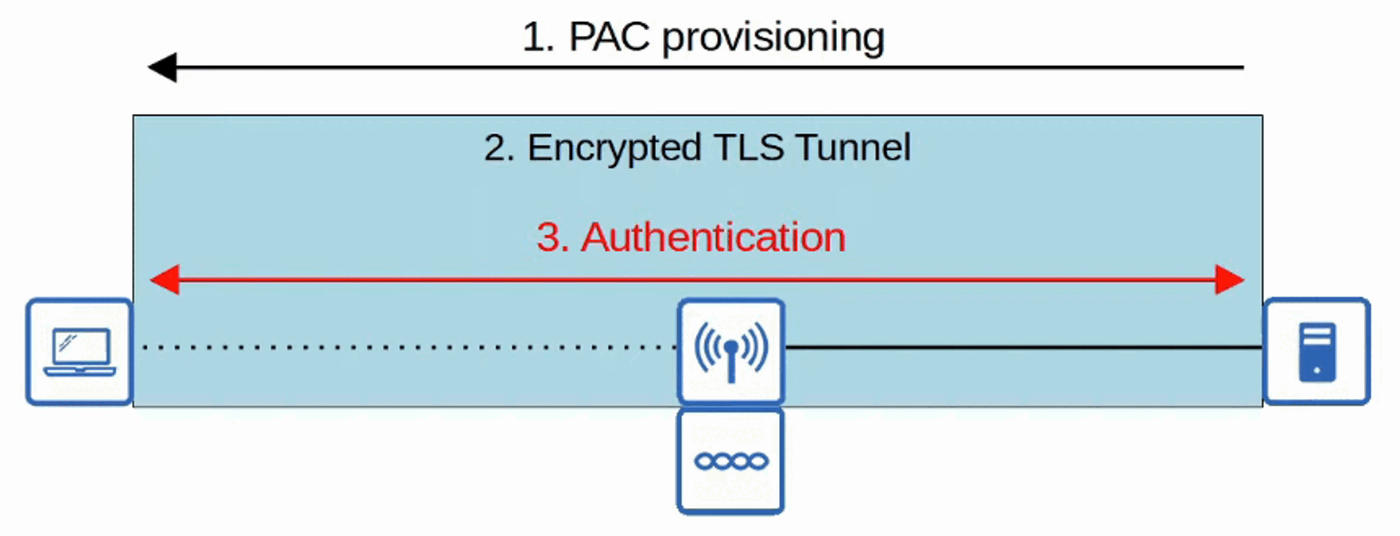
\includegraphics[keepaspectratio,alt={image}]{images/60-wireless-security/img-006.png}}
\end{figure}

\begin{itemize}
\tightlist
\item
  PEAP (PROTECTED EAP)

  \begin{itemize}
  \tightlist
  \item
    Like EAP-FAST, PEAP involves establishing a SECURE TLS TUNNEL
    between the CLIENT and SERVER
  \item
    Instead of a PAC, the SERVER has a DIGITAL CERTIFICATE
  \item
    The CLIENT uses this DIGITAL CERTIFICATE to AUTHENTICATE the SERVER
  \item
    The CERTIFICATE is also used to establish a TLS TUNNEL
  \item
    Because only the SERVER provides a CERTIFICATE for AUTHENTICATION,
    the CLIENT must still be AUTHENTICATED within the SECURE TUNNEL

    \begin{itemize}
    \tightlist
    \item
      Example: MS-CHAP (Microsoft Challenge-Handshake Authentication
      Protocol)
    \end{itemize}
  \end{itemize}
\end{itemize}

\begin{figure}
\centering
\pandocbounded{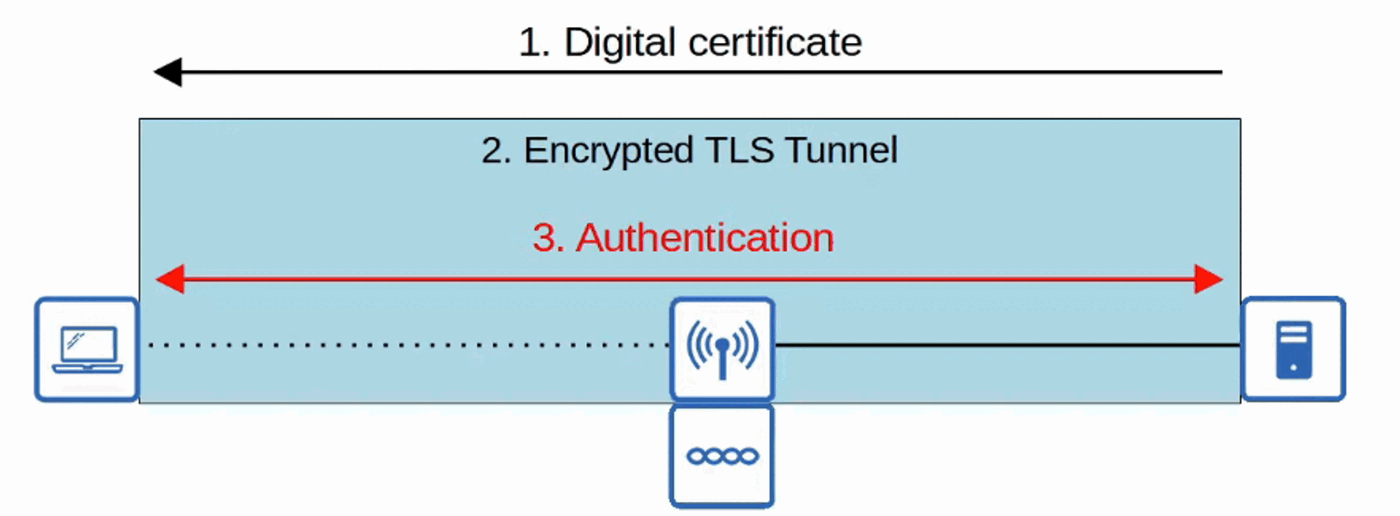
\includegraphics[keepaspectratio,alt={image}]{images/60-wireless-security/img-007.png}}
\end{figure}

\begin{itemize}
\tightlist
\item
  EAP-TLS (EAP TRANSPORT LAYER SECURITY)

  \begin{itemize}
  \tightlist
  \item
    Whereas PEAP only requires the AS to have a CERTIFICATE, EAP-TLS
    requires a CERTIFICATE on the AS and on every single CLIENT
  \item
    EAP-TLS is the MOST SECURE WIRELESS AUTHENTICATION method, but it is
    more difficult to implement than PEAP because every CLIENT DEVICE
    needs a CERTIFICATE
  \item
    Because the CLIENT and SERVER AUTHENTICATE each other with DIGITAL
    CERTIFICATES, there is no need to AUTHENTICATE the CLIENT within the
    TLS TUNNEL
  \item
    The TLS TUNNEL is still used to exchange ENCRYPTION KEY information
    (ENCRYPTION methods will be discussed next)
  \end{itemize}
\end{itemize}

\begin{figure}
\centering
\pandocbounded{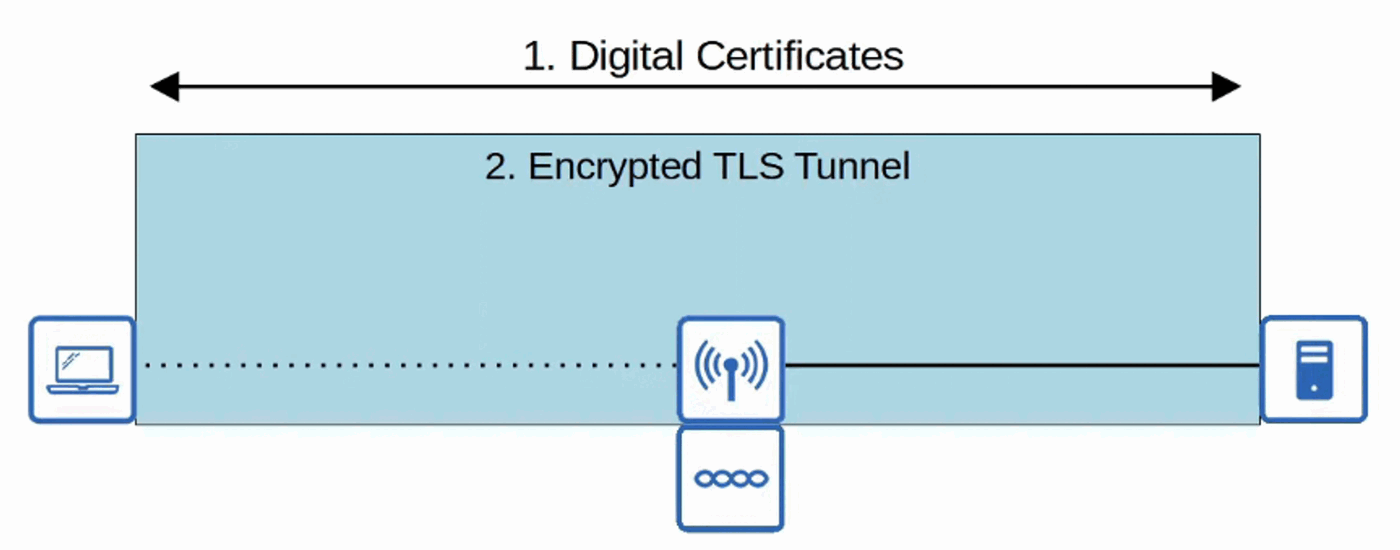
\includegraphics[keepaspectratio,alt={image}]{images/60-wireless-security/img-008.png}}
\end{figure}

\section{Encryption / Integrity
Methods}\label{encryption-integrity-methods}

\begin{itemize}
\tightlist
\item
  TKIP (Temporal Key Integrity Protocol)

  \begin{itemize}
  \tightlist
  \item
    WEP was found to be vulnerable, but WIRELESS hardware at the time
    was built to use WEP
  \item
    A temporary solution was needed until a new STANDARD was created and
    a new HARDWARE was built
  \item
    TKIP adds various SECURITY FEATURES:

    \begin{itemize}
    \tightlist
    \item
      A MIC (Message Integrity Check) is added to protect the integrity
      of messages
    \item
      A KEY MIXING ALGORITHM is used to create a unique WEP key for
      every frame
    \item
      The INITIALIZATION VECTOR is doubled in length from 24 bits to 48
      bits, making BRUTE-FORCE attacks much more difficult
    \item
      The MIC includes the SENDER MAC ADDRESS to identify the FRAME's
      SENDER
    \item
      A TIMESTAMP is added to the MIC to prevent replay attacks. Replay
      attacks involved re-resending a FRAME that has already been
      transmitted
    \item
      A TKIP SEQUENCE NUMBER is used to keep track of FRAMES sent from
      each SOURCE MAC ADDRESS. This also protects against REPLAY ATTACKS
    \end{itemize}
  \end{itemize}
\end{itemize}

** You probably don't need to memorize ALL of the above features

** TKIP is used in WPA version 1, which will be discussed in the next
section

\begin{itemize}
\tightlist
\item
  CCMP (Counter / CBC-MAC Protocol)

  \begin{itemize}
  \tightlist
  \item
    CCMP was developed after TKIP and is more SECURE
  \item
    It is used in WPA2
  \item
    To use CCMP, it must be supported by the DEVICE'S hardware.
  \item
    Old hardware built only to use WEP / TKIP cannot use CCMP
  \item
    CCMP consists of TWO DIFFERENT ALGORITHMS to provide ENCRYPTION and
    MIC :

    \begin{itemize}
    \tightlist
    \item
      AES (Advanced Encryption Standard) COUNTER MODE ENCRYPTION

      \begin{itemize}
      \tightlist
      \item
        AES is the MOST SECURE ENCRYPTION PROTOCOL currently available.
      \item
        Widely used all over the world
      \item
        There are multiple MODES of operation for AES.
      \item
        CCMP uses ``COUNTER MODE''
      \end{itemize}
    \item
      CBC-MAC (CIPHER BLOCK CHAINING MESSAGE AUTHENTICATION CODE)

      \begin{itemize}
      \tightlist
      \item
        Used as a MIC to ENSURE the INTEGRITY of MESSAGES
      \end{itemize}
    \end{itemize}
  \end{itemize}
\item
  GCMP (GALOIS / COUNTER MODE PROTOCOL)

  \begin{itemize}
  \tightlist
  \item
    GCMP is MORE SECURE and EFFICIENT than CCMP
  \item
    Its increased efficiency allows higher data throughput than CCMP
  \item
    It is used in WPA3
  \item
    GCMP consists of TWO ALGORITHMS:

    \begin{itemize}
    \tightlist
    \item
      AES COUNTER MODE ENCRYPTION
    \item
      GMAC (GALOIS MESSAGE AUTHENTICATION CODE)

      \begin{itemize}
      \tightlist
      \item
        Used as a MIC to ENSURE the INTEGRITY of MESSAGE
      \end{itemize}
    \end{itemize}
  \end{itemize}
\end{itemize}

\section{Wi-Fi Protected Access (WPA)}\label{wi-fi-protected-access-wpa}

\begin{itemize}
\tightlist
\item
  The WI-FI Alliance has developed THREE WPA CERTIFICATIONS for WIRELESS
  DEVICES:

  \begin{itemize}
  \tightlist
  \item
    WPA
  \item
    WPA2
  \item
    WPA3
  \end{itemize}
\item
  To be WPA-CERTIFIED, EQUIPMENT must be TESTED in authorized testing
  labs
\item
  All of the above support TWO AUTHENTICATION MODES:

  \begin{itemize}
  \tightlist
  \item
    PERSONAL MODE :

    \begin{itemize}
    \tightlist
    \item
      A PRE-SHARED KEY (PSK) is used for AUTHENTICATOIN
    \item
      When you connect to a home WI-FI NETWORK, enter the PASSWORD and
      are AUTHENTICATED, that is PERSONAL MODE
    \item
      This is common in small NETWORKS
    \item
      The PSK itself is NOT sent over the air
    \item
      A FOUR-WAY HANDSHAKE is used for AUTHENTICATION and the PSK is
      used to GENERATE ENCRYPTION KEYS
    \end{itemize}
  \item
    ENTERPRISE MODE :

    \begin{itemize}
    \tightlist
    \item
      802.1X is used with an AUTHENTICATION SERVER (RADIUS SERVER)
    \item
      No specific EAP METHOD is specified, so all are supported (PEAP,
      EAP-TLS, etc)
    \end{itemize}
  \end{itemize}
\end{itemize}

\section{WPA}\label{wpa}

\begin{lstlisting}
- The WPA CERTIFICATION was developed after WEP was proven to be vulnerable and includes the following PROTOCOLS:
    - TKIP (based on WEP) provides ENCRYPTION / MIC
    - 802.1X AUTHENTICATION (ENTERPRISE MODE) or PSK (PERSONAL MODE)

WPA2

- Was released in 2004 and includes the following PROTOCOLS:
    - CCMP provides ENCRYPTION / MIC
    - 802.1X AUTHENTICATION (ENTERPRISE MODE) or PSK (PERSONAL MODE)

WPA3

- Was released in 2018 and includes the following PROTOCOLS:
    - GCMP provides ENCRYPTION / MIC
    - 802.1X AUTHENTICATION (ENTERPRISE MODE) or PSK (PERSONAL MODE)

    - WPA3 also provides several additional security features:
        - PMF (PROTECTED MANAGEMENT FRAMES)
            - Protecting 802.11 MANAGEMENT FRAMES from eavesdropping / forging
        - SAE (SIMULTANEOUS AUTHENTICATION OF EQUALS)
            - Protects the four-way handshake when using PERSONAL MODE AUTHENTICATION
        - FORWARD SECRECY
            - Prevents DATA from being DECRYPTED after it has been transmitted over the air so an ATTACKER can’t capture WIRELESS FRAMES and then try to DECRYPT them later
\end{lstlisting}
